En los lotes de 50 cajas de los productos producidos por una determinada empresa producidos durante un determinado período, con un total de $n = 100$ cajas, se ha observado el número de piezas defectuosas, presentando ésta un total de $k = 11$ modalidades, cuya distribución de frecuencias viene representado en la siguiente tabla:
\begin{center}
	\begin{table}[htbp]
		\begin{center}
			\begin{tabular}{|r|r|r|r|r|r|r|}
				\hline
				\multicolumn{1}{|l|}{$x_{i}$} & \multicolumn{1}{l|}{$n_{i}$} & \multicolumn{1}{l|}{$N_{i}$} &
				\multicolumn{1}{l|}{$x_{i}n_{i}$} & \multicolumn{1}{l|}{$n_{i}|x_{i} - \bar x|$} & \multicolumn{1}{l|}{$n_{i}|x_{i} - Me|$} & \multicolumn{1}{l|}{$n_{i}(x_{i} - \bar x)^2$} \\ \hline
				0 & 6 & 6 & 0 & 26,16 & 27,00 & 114,06 \\ \hline
				1 & 9 & 15 & 9 & 30,24 & 31,50 & 101,61 \\ \hline
				2 & 10 & 25 & 20 & 23,60 & 25,00 & 55,70 \\ \hline
				3 & 11 & 36 & 33 & 14,96 & 16,50 & 20,35 \\ \hline
				4 & 14 & 50 & 56 & 5,04 & 7,00 & 1,81 \\ \hline
				5 & 16 & 66 & 80 & 10,24 & 8,00 & 6,55 \\ \hline
				6 & 16 & 82 & 96 & 26,24 & 24,00 & 43,03 \\ \hline
				7 & 9 & 91 & 63 & 23,76 & 22,50 & 62,73 \\ \hline
				8 & 4 & 95 & 32 & 14,56 & 14,00 & 53,00 \\ \hline
				9 & 3 & 98 & 27 & 13,92 & 13,50 & 64,59 \\ \hline
				10 & 2 & 100 & 20 & 11,28 & 11,00 & 63,62 \\ \hline
			\end{tabular}
		\end{center}
	\end{table}	
	
\end{center}

\subproblem
Calcular el n{\'u}mero medio de piezas defectuosas por caja.

La variable estadística observada es discreta, presentando un total de 11 modalidades: 0, 1, 2, 3, 4, 5, 6, 7, 8, 9 y 10. En este caso, de las medias de las que disponemos, la única con significado estadístico es la aritmética, cuya expresión matemática viene determinada por:

	$$\bar{x} = \frac{1}{n} \sum_{i=1}^{k}x_{i} n_{i}$$

De la tabla podemos obtener, teniendo también en consideración que $n=100$ cajas, que $\bar{x} = 4,36 \approx 4$ piezas. Esto es, en cada lote examinado, cabe esperar un total de 4 piezas defectuosas de media, aunque para cálculos empleamos 4,36 piezas. \\


\subproblem 
?`Cuantas piezas defectuosas se encuentran m{\'a}s frecuentemente en las
cajas examinadas?

La medida estadística que proporciona información sobre el número de piezas defectuosas que más habitualmente se puede esperar de una caja es la moda. Se define como $Mo = max(x_{i})$, con $i=1,2,3,...,k$. En este caso, se presentan dos modalidades que presentan la misma frecuencia absoluta. Por tanto, podemos afirmar que hay dos valores de moda en esta distribución, siendo más frecuente encontrar un total de 5 y 6 piezas defectuosas por lote examinado. \\

% Revisar concepto de mediana.
\subproblem
?`Cu{\'a}l es el n{\'u}mero mediano de piezas defectuosas por caja?

La mediana se define como un valor que divide a una determinada población en dos subgrupos con el mismo número de individuos: una de ellas cuyos individuos pertenecen a una modalidad cuya frecuencia absoluta es inferior a la mediana y otra con frecuencias absolutas superiores.

Para determinar la mediana en esta distribución de frecuencias, representamos la curva de distribución de la variable estadística: 

\begin{center}
	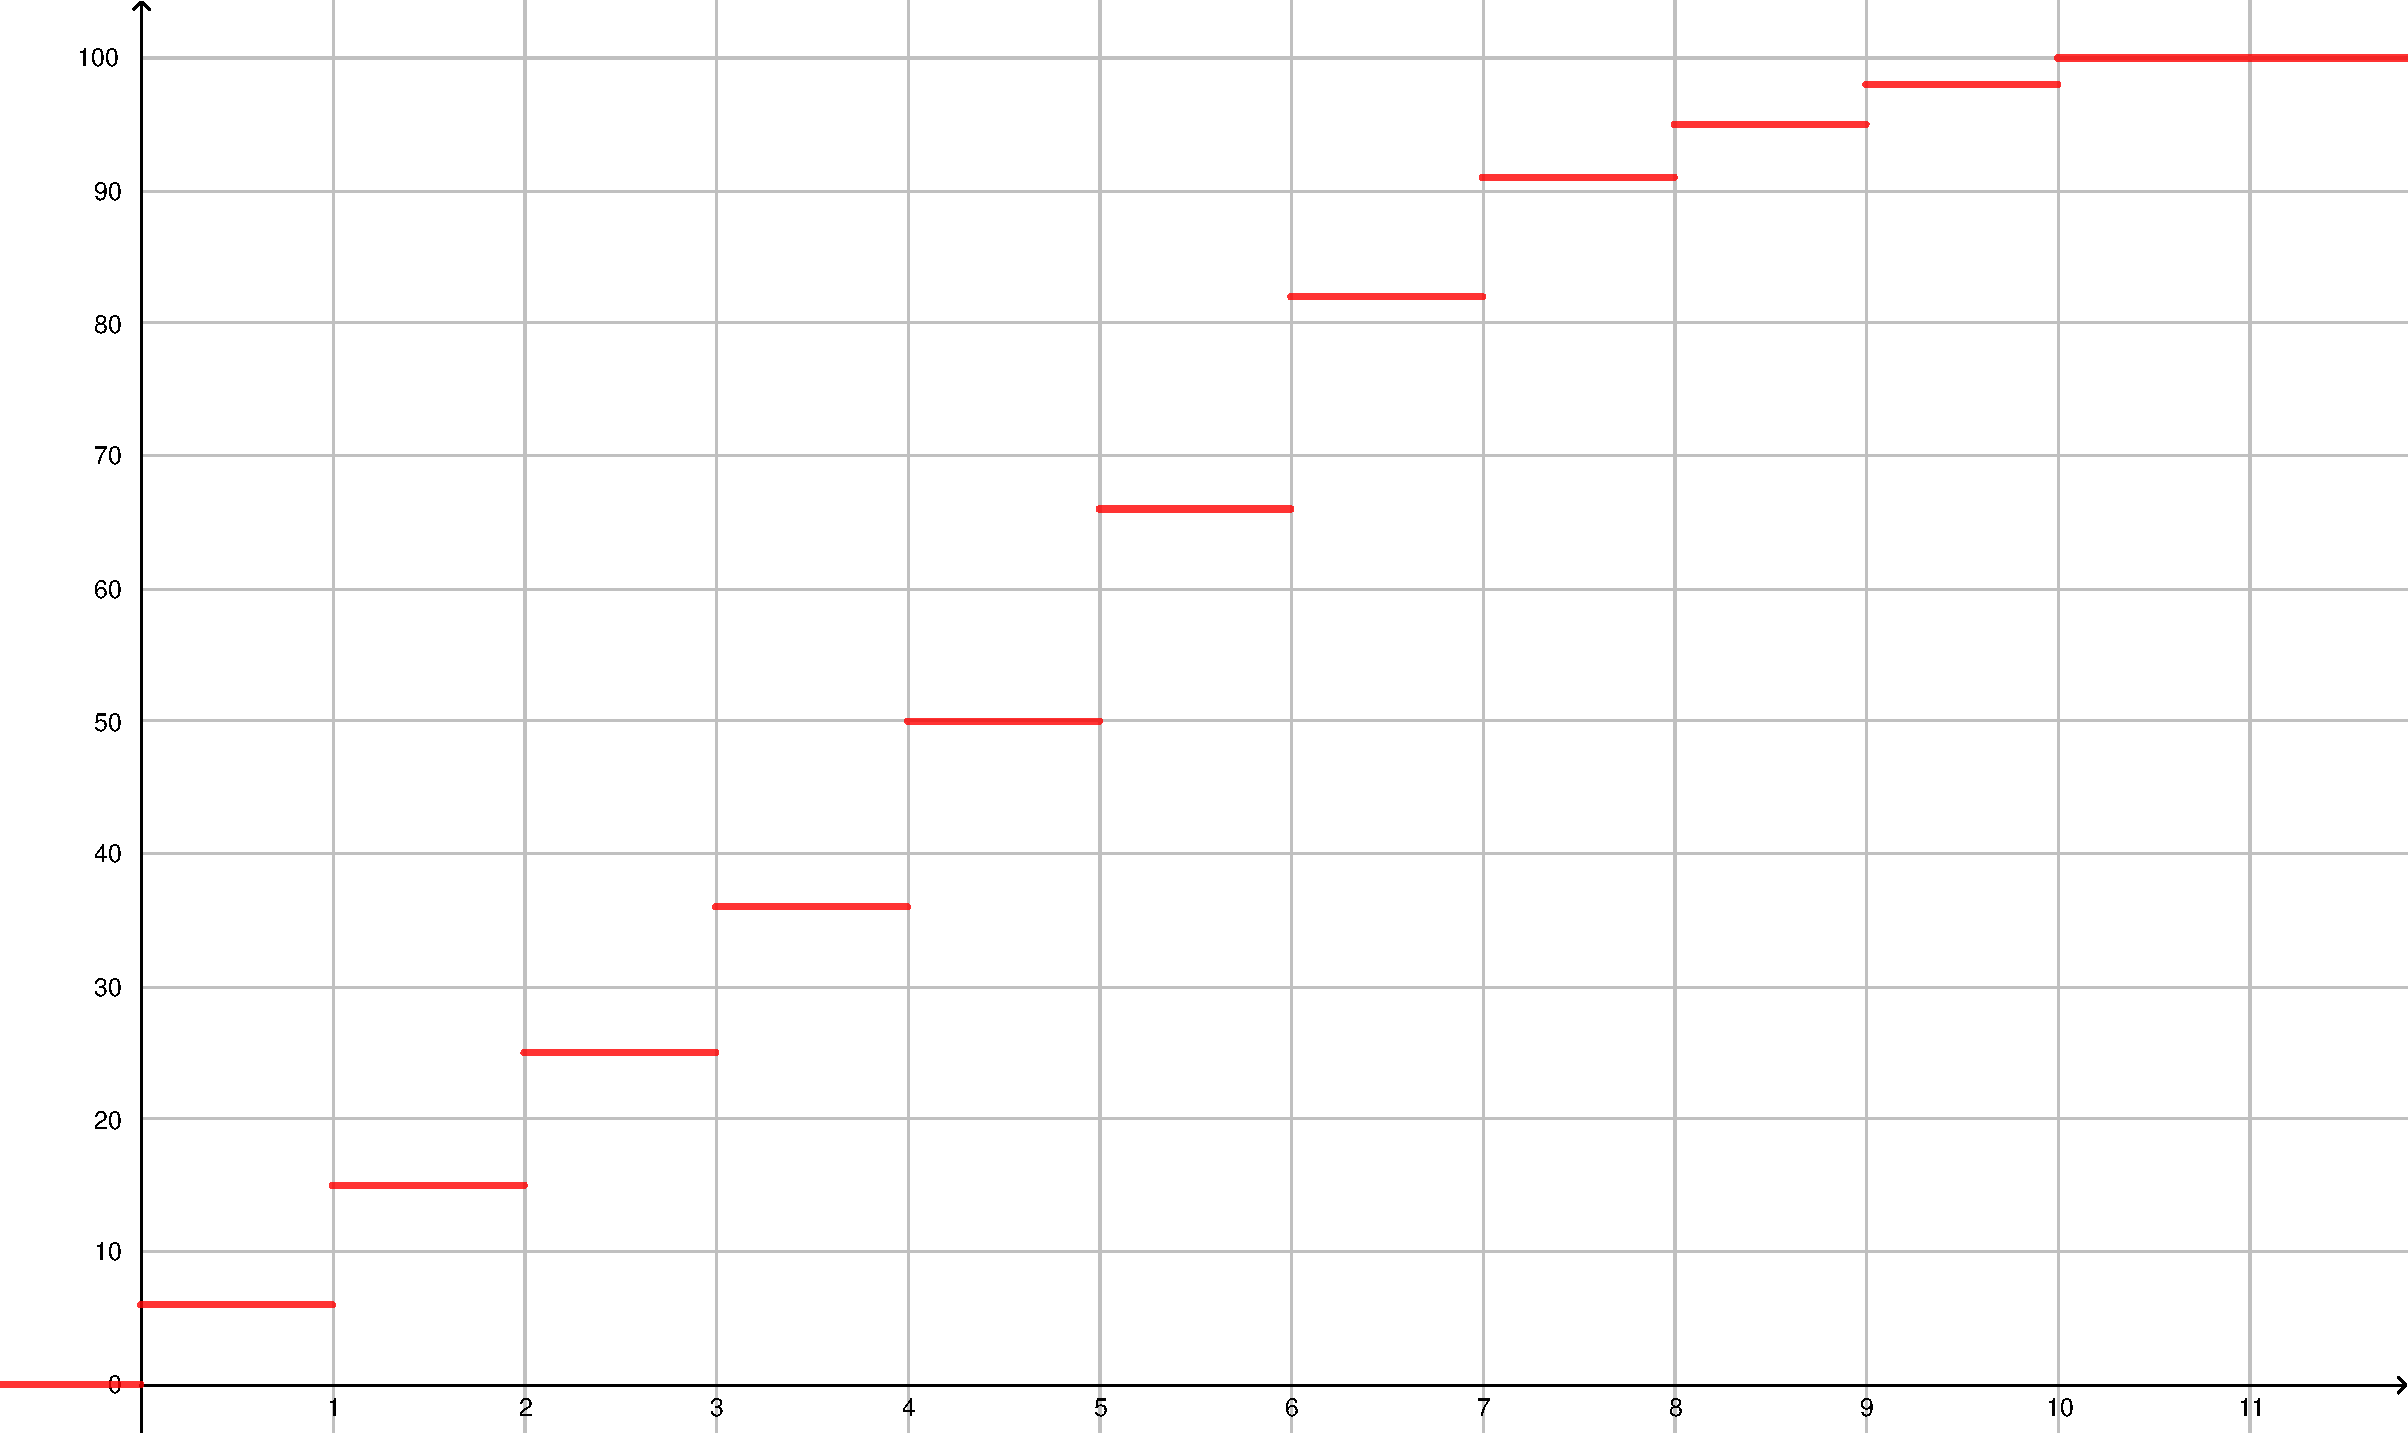
\includegraphics[scale=.35]{ejercicio-4-grafica.pdf}
\end{center}

Observamos que $\frac{n}{2} = 50$, coincidiendo justamente con el valor $F(x_{5}) = n/2$. Conviene pues tomar la media aritmética entre $x_{5}$ y $x_{6}$, de donde $Me = 4,5$ piezas defectuosas. \\

\subproblem
Calcular los cuartiles de la distribuci{\'o}n. Interpretarlos.

El cuartil es una medida que permite caracterizar el porcentaje de individuos de la población cuya variable estadística observada es inferior al $25\%, 50\%, 75\%$ de toda la población, respectivamente. Su cálculo es análogo al de la media (únicamente hay que sustituir $\frac{n}{2}$ por las fracciones correspondientes). De esta forma, deducimos las siguientes medidas:

\begin{itemize}
	\item $Q_{1} = 2,5$ piezas. Representa que un $25\%$ de los lotes analizados poseen una cantidad de productos defectuosos inferiores o iguales a 2,5 piezas.
	
	\item $Q_{2} = 4,5$ piezas. Representa que un $50\%$ de los lotes analizados poseen una cantidad de productos defectuosos inferiores o iguales a 4,5 piezas.
	
	\item $Q_{3} = 6$ piezas. Representa que un $75\%$ de los lotes analizados poseen una cantidad de productos defectuosos inferiores o iguales a 6 piezas.
\end{itemize}

\subproblem
Calcular los deciles de orden 3 y 7. Interpretarlos.

El decil tiene un significado análogo a la de los cuartiles. Por tanto, el decil es una medida que permite caracterizar el porcentaje de individuos de la población cuya variable estadística observada es inferior al $10\%, 20\%,..., 90\%$ de toda la población. Su cálculo es, nuevamente, análogo a los casos anteriores: 

\begin{itemize}
	\item $D_{3} = 3$ piezas. Representa que un $30\%$ de los lotes analizados poseen una cantidad de productos defectuosos inferiores o iguales a 3 piezas.
	
	\item $D_{7} = 6$ piezas. Representa que un $70\%$ de los lotes analizados poseen una cantidad de productos defectuosos inferiores o iguales a 6 piezas. \\
\end{itemize}


\subproblem
Cuantificar la dispersi{\'o}n de la  distribuci{\'o}n utilizando diferentes
medidas, interpretando los resultados  y se{\~n}alando las ventajas e
inconvenientes de cada una.

Algunas medidas de dispersión que podemos tomar sobre la variable estadística observada son las siguientes:

\begin{itemize}
	
	\item Recorrido. Es la magnitud que determina la anchura total de la muestra tomada (esto es, toma la diferencia entre el valor más alto tomado de la variable y el menor valor observado). Su ventaja es que tiene un significado concreto, pero su inconveniente es que varía mucho con fluctuaciones muestrales. En este caso, su valor es $R = 10$ piezas. Esto quiere decir que hay una variación de 10 productos defectuosos entre los datos de la muestra.
	
	\item Recorrido intercuartílico. Es la magnitud que indica la longitud del intervalo que contiene al $50\%$ central de los datos observados. Su virtud es que no varía mucho con fluctuaciones muestrales, pero su inconveniente es que no toma en consideración todos los datos de la población observada. En este caso, su valor es $R_{I} = 3,5$ piezas. Ello quiere decir que, del $50\%$ central de la muestra, hay, a lo sumo, una diferencia de 3,5 piezas defectuosas entre ellos.
	
	% Poner ventajas e inconvenientes.
	\item Desviación absoluta media respecto a la media aritmética. Indica cómo están los datos distribuidos en función del valor promedio (la media aritmética). Su ventaja es que tiene un significado preciso, pero presenta el inconveniente de que varía mucho en función de fluctuaciones estadísticas (puesto que en su cálculo interviene la media aritmética). Su valor es, en este caso, $D_{\bar x} = 2$ piezas. Representa que los individuos de la población muestran una diferencia de media de 2 piezas defectuosas respecto a la media aritmética.
	
	\item Desviación absoluta media respecto a la mediana. Es la medida que representa la media de las distancias de los valores presentados durante la muestra respecto al $50\%$. Presenta la ventaja de que tiene un significado preciso, pero no es fácil de calcular. Su valor es $D_{Me} = 2$ piezas, en este caso. Esto significa que los individuos presentan, respecto a la mediana, una diferencia de 2 piezas defectuosas.
	
	\item Varianza. Es una medida que representa la variabilidad de una serie de datos respecto a su media. Presenta la ventaja de que en su cálculo intervienen todos las modalidades observadas de la variable estadística, pero su inconveniente es que su valor es sensible a fluctuaciones muestrales. Su valor numérico, en este caso, es $Var(X) = 5,85$ piezas al cuadrado. No aporta información relevante, pero se usará para calcular la desviación típica, que sí proporciona mayor información. 
	
	\item Desviación típica. Es una medida que proporciona información sobre el margen óptimo de diferencia entre los valores medidos de la variable respecto de la media aritmética. Su principal ventaja es que fluctúa poco con variaciones extremas de la muestra, pero tiene el inconveniente de que requiere gran capacidad de cómputo para poder calcularse. Su valor es, en este caso, $\sigma_{x} = 2,42$ piezas. Su significado es que, respecto a la media, la diferencia óptima que se debería encontrar en la distribución es de 2,42 piezas.
	
	\item Recorrido relativo. Informa sobre el recorrido de la variable respecto de su media aritmética. Su ventaja es que es fácil de calcular, pero tiene la desventaja de que varía mucho con las fluctuaciones estadísticas. En este caso, su valor es $R_{R} = 0,8$. Informa que la amplitud de las modalidades tomadas oscila en torno a 0,8 veces la media arimética.
	
	%\item Recorrido semi-intercuartílico. 
	
	\item Coeficiente de variación. Representa la desviación típica de la muestra en función de la media aritmética. Su principal virtud es que comparar el grado de dispersión entre diferentes variables estadísticas, pero tiene el inconveniente de que no es válida para todas las variables estadísticas (no sería válida para aquellas con $\bar x = 0$ u). Su valor es, en este caso, $C.V.(X) = 0,55$. Se trata de una medida adimensional. Dado que este coeficiente es inferior a 0.8, deducimos que la distribución es homogénea. 
	
	%\item Índice de dispersión respecto a la mediana. 
\end{itemize}

%$Var(X) = 5,85$ (no proporciona información relevante) piezas al cuadrado.



%$R_{SI} = 0,41$.
%$V_{Me} = 0,44$.